%!TEX root = ../report.tex
\documentclass[report.tex]{subfiles}
\begin{document}

    \chapter{Additional Content}

        \section{Glossary}
        \begin{itemize}
                
                \item  Robot learning - Deals with algorithms, methods, and methodologies that enable a robot to master new tasks such as navigation, manipulation, and object classification.
                \item Interactive machine learning (IML)  -An area at the intersection of Machine Learning and Human-Computer/Machine Interaction, where human interaction is central to the learning process.
                \item Reinforcement learning (RL) - A branch of machine learning focused on how an autonomous agent learns sequential decisions in an uncertain environment by maximizing a cumulative reward
                \item Learning from feedback - Involves human feedback provided with the intention of evaluating (critiquing) the robot's actions
                \item Learning from demonstrations (LfD) - Methods that assume demonstrations, typically state-action pairs, are the sole teaching signals available to the learner
                \item Inverse Reinforcement Learning (IRL) - A common approach in imitation learning that aims to deduce an unknown reward function from a set of demonstrations and subsequently find the optimal policy based on that learned reward function.
                \item Learning from instructions -  Formulated as the process of mapping instructions, often in natural language, to a sequence of executable actions.
                \item Human teaching strategies - The main methods and models that enable humans to teach embodied social agents, such as social robots, using natural interaction. 
                \item Human Robot Interaction (HRI) -It is a field that focuses on the interactions between humans and robots.
                \item Interactive Task Learning (ITL) -  A primary application area for interactive robot learning algorithms, focused on developing agents capable of learning tasks through natural interaction with a human instructor. 
                \item Markov Decision Process (MDP) - A framework used to model environments in reinforcement learning, characterized by a tuple including state space, action space, state-transition probability function, reward function, and a discount factor. 
                \item machine learning - A field of artificial intelligence that uses statistical techniques to give computer systems the ability to "learn" from data, without being explicitly programmed.
                \item imitation learning : a robot learning approach where an agent acquires new skills by observing and replicating demonstrations from a human or another expert, instead of learning through trial and error or explicit programming.
            \end{itemize}


            
        \section{Sources}
            \subsection{List of searched journals}
            \begin{itemize}
                \item {IEEE Transactions on Neural Networks and Learning Systems  } 
                \item {IEEE Robotics and Automation Letters - High-impact journal for cutting-edge robotics research.} 
                \item {IEEE Transactions on Industrial Electronics - Important venue for industrial applications of interactive robot learning.}
                
            \end{itemize}
            
            \subsection{List of searched conference proceedings}
            \begin{itemize}
                \item {IEEE/RSJ International Conference on Intelligent Robots and Systems (IROS) } 
                \item {IEEE International Conference on Robotics and Automation (ICRA)} 
                \item {ACM/IEEE International Conference on Human-Robot Interaction (HRI)} 
                \item {IEEE International Symposium on Robot and Human Interactive Communication (RO-MAN)} 
            \end{itemize}
            
    
        \section{Keywords and keyword combinations used for search}
        \begin{itemize}
            \item {Primary Keywords : Interactive robot learning,Human-robot interaction,Reinforcement learning,Imitation learning,Robot learning from demonstration,Active learning robotics,Social robotics,}
            \item {Core Learning Methodologies : "Interactive robot learning" AND "reinforcement learning", "Robot learning" AND "human feedback" , "Active learning" AND "robotics", "Inverse reinforcement learning" AND "human robot" }
        \end{itemize}
        
        \section{List of most important conferences}
        \begin{itemize}
            \item  {IEEE/RSJ International Conference on Intelligent Robots and Systems (IROS)}
            \item   {IEEE International Symposium on Robot and Human Interactive Communication (RO-MAN)}
            \item {ACM Designing Interactive Systems Conference (DIS)}
            \item {IEEE International Conference on Consumer Electronics (ICCE)}
            \item { International Conference on Innovative Mechanisms for Industry Applications (ICIMIA)}
            \item {International Conference on Ubiquitous Robots (UR)}
        \end{itemize}
        \section{List of most important journals and magazines}
        \begin{itemize}
            \item \textbf{Tier 1 Journals (Highest Impact)}
            \item {ACM Computing Surveys}
            \item {Artificial Intelligence (Elsevier)}
            \item {IEEE Transactions on Cognitive and Developmental Systems}
    
            \item {IEEE Transactions on Automation Science and Engineering}
            \item {IEEE Access}
            \item {Scientific Reports (Nature Portfolio)}
            \item \textbf{Specialized Journals }
            \item {Sensors, Applied Sciences, Frontiers in Robotics and AI, Mechatronics, MethodsX}
            
            \section{List of most important Researchers and Research Labs}
            \item {Researchers:M. Chetouani, A.-L. Vollmer, T. D. Murphey, D. P. Losey, E. Rueckert, V. Kyrki, S. K. Kim, E. A. Kirchner, F. Kirchner, P. Doshi, A. Loutfi, A. Hussein, M. M. Gaber, E. Elyan, C. Jayne, J. Hua, L. Zeng, G. Li, Z. Ju, J. Lin, Z. Ma, R. Gomez, K. Nakamura, B. He, S. Ambhore, A.-M. Velentza, N. Fachantidis, I. Lefkos, A. Angleraud, Q. Houbre, R. Pieters, L. Hindemith, O. Bruns, A. M. Noller, N. Hemion, S. Schneider, Y. Kim, H. Jeon, B.-Y. Kang, A. T. Taylor, T. A. Berrueta, I. Tarakli, S. Vinanzi, A. D. Nuovo, I. Moreira, J. Rivas, F. Cruz, R. Dazeley, A. Ayala, B. Fernandes, S. Habibian, A. Alvarez Valdivia, L. H. Blumenschein, N. Feith, H. Chen, H. Beierling, R. Beierling, C. Arzate Cruz, T. Igarashi, S. Arora, N. Akalin }
    
            \item {Labs and  groups :Tampere University (Finland), University of Bremen/DFKI Robotics Innovation Center (Germany), Örebro University AASS Research Centre (Sweden), Vanderbilt University Robotics Lab (USA), University of Georgia AI Lab (USA), IEEE Robotics and Automation Society, ACM Computing Surveys, Fraunhofer Institute (Germany), University of Birmingham (UK), University of Portsmouth (UK), University of Lincoln (UK), Heriot-Watt University (UK), Tokyo Institute of Technology (Japan), Northwestern University (USA), Carnegie Mellon University (USA), University of Coimbra (Portugal), Griffith University (Australia), Federal University of Pernambuco (Brazil), University of Washington (USA) }
        \end{itemize}
        \section{Top 100 papers}
        The list of the top 100 papers is \href{https://drive.google.com/file/d/19iwr8xqD-wopxZIMe9OjLMB2xNGlfBga/view?usp=sharing} {here}.
        \section{Use Of AI Assistance}
        
            {AI tool Claude AI was used throughout the preparation of this report to support the writing
and organization process. Its primary functions were to proofread sections for grammatical accuracy
and to suggest alternative phrasing to improve clarity and flow. Additionally, AI assistance helped
structure the annotated bibliography, categorize selected papers, and insert relevant references based
on their methodological focus. All interpretations, evaluations, and conclusions presented in this
report are entirely the author’s own and have been carefully reviewed to ensure both accuracy and
originality}
        
        \clearpage 
        \section{Mindmap}
            \begin{figure}[h]
                \centering
                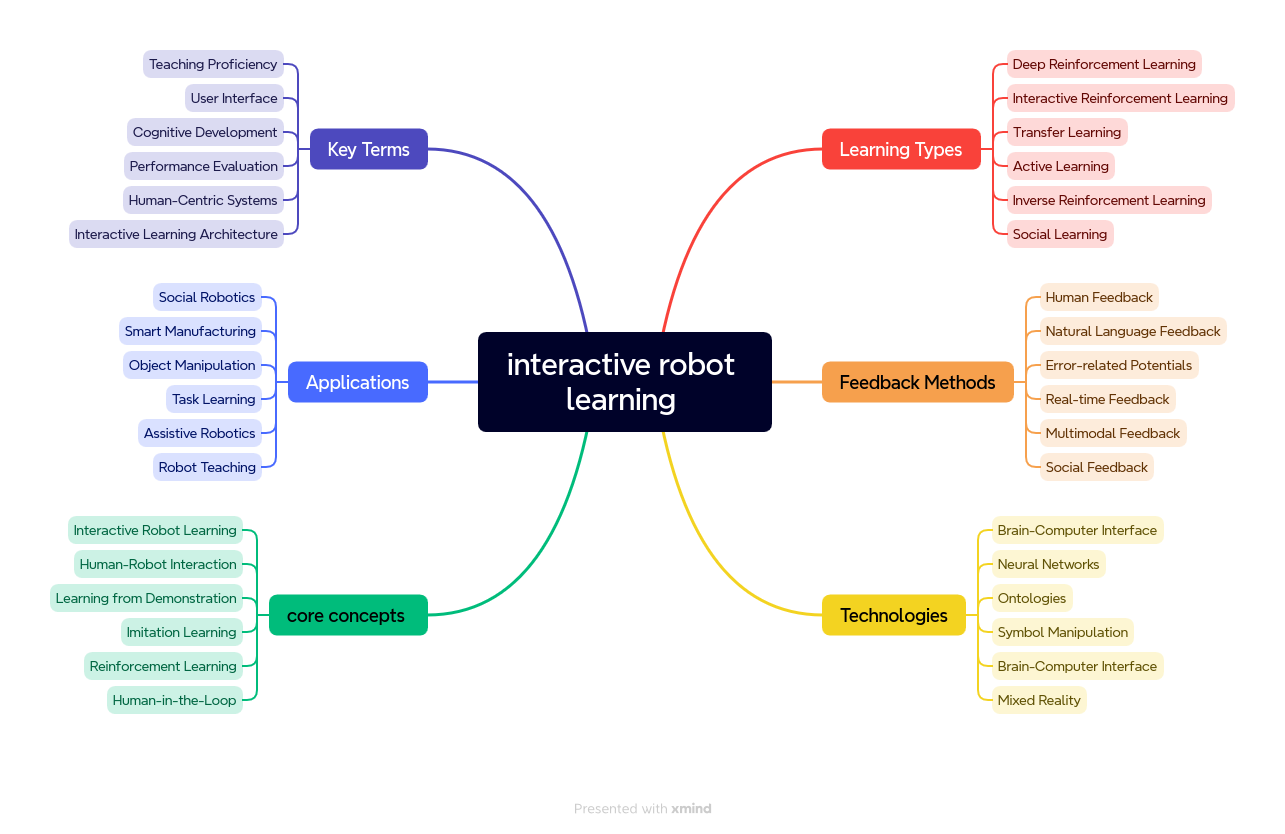
\includegraphics[width=0.8\textwidth]{images/Mind-Map.png} 
                \caption{Mind Map}
                \label{fig:your-label}
            \end{figure}
        \clearpage  


        %\addcontentsline{toc}{section}{Included Paper}
        
    


\end{document}
